%-------------------------------------------------------------------------------
% 请勿删除本注释
% Free Response Question 2
%
% 指引:
% 如在小问之前有通用问题描述,请放置于此
%-------------------------------------------------------------------------------

\question
A student is to design a circuit using a battery $\varepsilon$ with negligible internal resistance, two uncharged capacitors $C_{1}$ and $C_{2}$, a resistor $R$, and a switch $S$. The circuit should be set up so that when the switch is in one position, the battery will only charge capacitor $C_{1}$, and when in the second position, capacitor $C_{1}$ will discharge through capacitor $C_{2}$ and resistor $R$. % 请删除并替换本行,与上一行 \question 之间不要留空行

\begin{parts}

%-------------------------------------------------------------------------------
% 请勿删除本注释
% Part (a)
%
% 指引:
% 如在小问之前有通用问题描述,请放置于此
%-------------------------------------------------------------------------------

\part
Using the components shown below, draw a circuit diagram that represents a single circuit that will satisfy the criteria outlined above. % 请删除并替换本行,与上一行 \part 之间不要留空行

\begin{figure}[H]
\centering
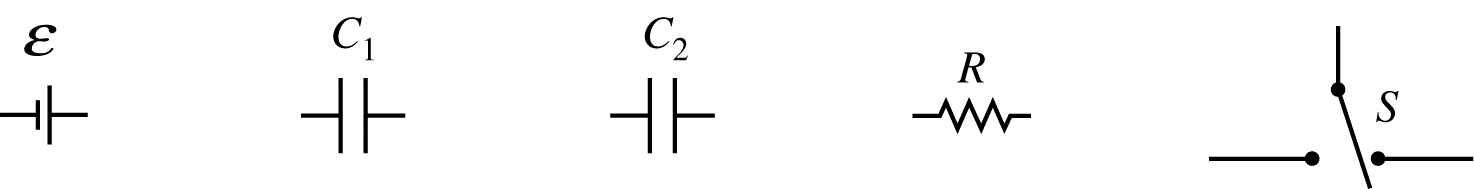
\includegraphics[scale=0.3]{images/img-019-027.png}
\end{figure}

%-------------------------------------------------------------------------------
% 请勿删除本注释
% Part (b)
%
% 指引:
% 如在小问之前有通用问题描述,请放置于此
%-------------------------------------------------------------------------------

The switch $S$ is initially in position to fully charge capacitor $C_{1}$. At time $t=0$, the switch is moved to the second position. The charge as a function of time for both capacitors after the switch is moved is plotted on the graph below.

\part
Label each box to indicate which graph corresponds to $C_{1}$ and $C_{2}$. % 请删除并替换本行,与上一行 \part 之间不要留空行

\begin{figure}[H]
\centering
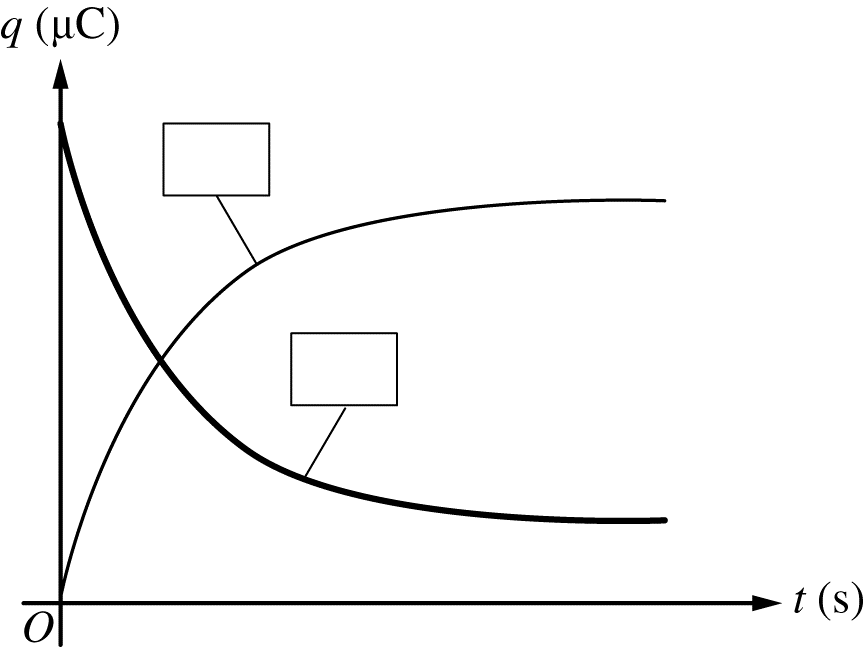
\includegraphics[scale=0.3]{images/img-019-028.png}
\end{figure}

%-------------------------------------------------------------------------------
% 请勿删除本注释
% Part (c)
%
% 指引:
% 如在小问之前有通用问题描述,请放置于此
%-------------------------------------------------------------------------------

The components of the circuit have the following values: $R=1000 \Omega, C_{1}=2.0 \mu \mathrm{F}, C_{2}=6.0 \mu \mathrm{F}, \varepsilon=12 \mathrm{~V}$.

\part
Calculate the following for a long time after the switch has been moved to the second position. % 请删除并替换本行,与上一行 \part 之间不要留空行
\begin{subparts}
\subpart The charges $q_{1}$ and $q_{2}$ stored on capacitors $C_{1}$ and $C_{2}$, respectively
\subpart The potential differences $V_{1}$ and $V_{2}$ across the capacitors $C_{1}$ and $C_{2}$, respectively
\end{subparts}

%-------------------------------------------------------------------------------
% 请勿删除本注释
% Part (d)
%
% 指引:
% 如在小问之前有通用问题描述,请放置于此
%-------------------------------------------------------------------------------

\part
Calculate the total energy dissipated in resistor $R$ during the time capacitor $C_{1}$ discharges. % 请删除并替换本行,与上一行 \part 之间不要留空行

%-------------------------------------------------------------------------------
% 请勿删除本注释
% Part (e)
%
% 指引:
% 如在小问之前有通用问题描述,请放置于此
%-------------------------------------------------------------------------------

\part
 % 请删除并替换本行,与上一行 \part 之间不要留空行
\begin{subparts}
\subpart Write, but do NOT solve, a differential equation that could be used to determine the time constant associated with the discharge of $C_{1}$.
\subpart Calculate the time constant associated with the discharge of $C_{1}$.
\end{subparts}

\end{parts}
